\documentclass[article,12pt,onesidea,4paper,english,brazil]{abntex2}

\usepackage{lmodern, indentfirst, nomencl, color, graphicx, microtype, lipsum}			
\usepackage[T1]{fontenc}		
\usepackage[utf8]{inputenc}		

\setlrmarginsandblock{2cm}{2cm}{*}
\setulmarginsandblock{2cm}{2cm}{*}
\checkandfixthelayout

\setlength{\parindent}{1.3cm}
\setlength{\parskip}{0.2cm}

\SingleSpacing

\begin{document}
	
	\selectlanguage{brazil}
	
	\frenchspacing 
	
	\begin{center}
		\LARGE PRODUÇÃO DE MORANGOS AUXILIADA PELA TECNOLOGIA ARDUÍNO PARA EXERCER O CONTROLE DE HUMIDADE DO SOLO, DO AR E DA TEMPERATURA\footnote{Área de Conhecimento CNPq/CAPES: Ciência da Computação com financiamento do IFRO - Campus Vilhena.}
		
		\normalsize
		Bruno Rover Dal Prá\footnote{Orientador, bruno.dalpra@ifro.edu.br, Campus Vilhena.} 
	Eberson Taynan Tomazelli\footnote{Colaborador, eberson\_taynan@hotmail.com, Campus Vilhena.} 
		José Leonardo Alves Leite\footnote{Bolsista, j.leonardo2012@hotmail.com, Campus Vilhena.} 
	\end{center}
	
	% resumo em português
	\begin{resumoumacoluna}
		Atualmente produtos eletrônicos eficientes, seja qual for sua aplicação, possuem um preço de mercado elevado. O presente projeto viabilizou um sistema de controle e análise avaliativa da irrigação. Onde será controlado e analisado a umidade do solo, do ar e a temperatura ambiente usando sensores e tecnologias de baixo custo. Serão primícias do projeto a utilização de tecnologias OpenSource(Código Aberto), com isso teremos um produto com um custo mais acessível atendendo um público hoje esquecido pelas empresas que desenvolvem estas tecnologias. A inovação consiste em utilizar os 3 parâmetros simultaneamente e através de um hardware com um software embarcado analisar os dados coletados pelos sensores e decidir a melhor hora de irrigar e amenizar a temperatura interna da estufa através de aspersores/nebulizadores. O cultivo escolhido para as primeiras análises foi o morango, por se tratar de uma cultura que necessita grande quantidade de defensivos agrícolas, sensível a mudanças climáticas e de umidade do solo. Este estudo está sendo realizado em uma casa de vegetação no setor rural do município de Vilhena – RO, medindo 6m de largura por 10m de comprimento e pé direito de 2,5m, utilizando irrigação por gotejamento e controle de temperatura por nebulizadores. O hardware e o software foram testados em laboratório obtendo grandes resultados e necessitando apenas da validação dos mesmo em campo. Com testes em campo, esperamos avaliar os dados de produção, incidência de doenças e análise de consumo de água. Assim, verificando se o controle dessas variáveis influencia no desenvolvimento da planta.
		\vspace{\onelineskip}
		
		\noindent
		\textbf{Palavras-chave}: Eletrônica, Estufa, Nebulizador.
	\end{resumoumacoluna}
	
	\textual
	
	\section*{Introdução}
	
	A diminuição de custos e o aumento da produção contribuem para um mercado consumidor mais eficiente e próspero. Nesse sentido, o morango tem mostrado ser um fruto de grande valia no decorrer de sua produção, podendo tornar-se rentável quando o produtor faz seu correto acompanhamento. A principal vantagem na produção do morango por elevação é que nos meses mais quentes a planta não deixa de produzir e a muda pode ser cultivada por dois ou três anos (PAGNONCELLI, 2015).
	
	O mundo contemporâneo é embasado na produção de alimentos em larga escala, assim conseguirmos manter a renda e a produção de capital a elevado crescimento. No entanto, a incorreta produção de frutos, sem controle e gerenciamento adequado, ocasionando em perdas desde a plantação até a venda tem causado preocupações e conflitos.
	
	Em propriedades familiares possui destaque na alta rentabilidade em sua área cultivada, podendo a produção ser destinada ao mercado de frutas frescas e à industrialização (RESENDE, 1999).
	
	Um bom exemplo refletido é a falta administrativa no controle de qualidade dos produtos em todo seu processo produtivo. Quando falamos em qualidade da mercadoria, analisa-se a condição física e saborosa que este se encontra, devendo ser investigado desde o processo de produção até a chegada na mesa do consumidor. Nesse sentido, o presente projeto tem por objetivo, através do controle de irrigação e acompanhamento térmico da plantação, radicalizar o uso de agrotóxicos nas plantações de morango e consequentemente gerar um hábito saudável aos consumidores, além de estimular a pesquisa e inovação tecnológica promovida pelo mesmo, ao decorrer das aplicações em eletrônica digital na plataforma Arduíno.
	
	\section*{Material e Método}
	
	Este estudo foi realizado em uma casa de vegetação no setor rural do município de Vilhena – RO. A classe de solo predominante no município são os Latosolos Vermelho Amarelo Distrófico, com textura argilosa (CARVALHO et al, 2011). Foi utilizada uma casa de vegetação com 6m de largura por 10m de comprimento e pé direito de 2,5m (figura 3), onde serão cultivados os morangos. Também foi preparado dois canos de 6 (seis) metros de largura e 20 (vinte) milímetros de diâmetro que serão plantados o cultivar. Será instalado os canos do cultivo da fruta, uma tomada para o fornecimento de energia elétrica para alimentação dos sistemas de controle. Também foi instalado uma rede de água para
	3
	suprir a irrigação das plantas e sistema de controle de temperatura que utilizará sistema de nebulização para o controle da temperatura interna da casa de vegetação.
	As plataformas (softwares) usadas para construir o software foram o Eclipse para codificação, Bizagi Process Modeler para elaboração dos fluxogramas relacionados aos processos executados no software desenvolvido e o Protheus, no qual, neste último, importamos algumas bibliotecas do Arduíno para o seu Banco de Dados podendo simular o resultado do estudo.
	Foi realizada a construção de um software que realize o controle dos parâmetros descritos na pesquisa conforme os fluxogramas das figuras 1 e 2.
	
	O modelo da placa utilizada será o Arduíno Mega 2560 que será realizará o controle dos parâmetros mencionados e com a utilização de interfaces de potência que utilizando as análises dos sensores decidirá quando deverão ser acionadas as bombas para controle da umidade do solo e nebulização interna da casa de vegetação.
		
	
	
	\section*{Resultados e Discussão}
	
	O projeto conseguiu expor as deficiências que a agricultura contemporânea do morango vem sofrendo, no qual, muitas plantações são perdidas pela falta de um cultivo, fertilização e irrigação corretas. Para Testezlaf (2010), quando ocorre o reaproveitamento hídrico, irrigando apenas ao redor da planta (irrigação localizada), diminui consideravelmente a evaporação direta da água do solo para a atmosfera, erradicando o desperdício dos recursos naturais e financeiros.
	
	\begin{figure}[h]
		\centering
		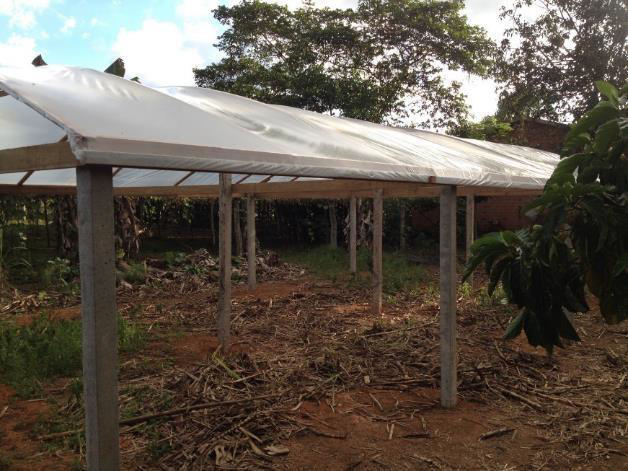
\includegraphics[width=.6\linewidth]{pip-156-01}
		\caption{Casa de vegetação Construídas. IFRO, 2015.}
	\end{figure} 

\begin{figure}[!h]
	\centering
	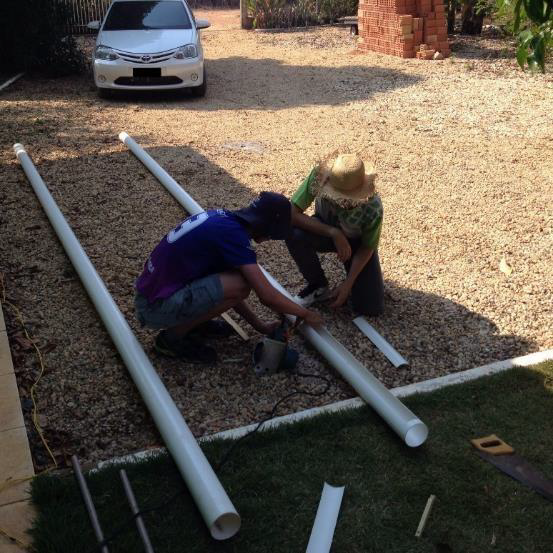
\includegraphics[width=.6\linewidth]{pip-156-02}
	\caption{Corte dos Canos. IFRO, 2015.}
\end{figure}

	
	Assim, em alguns meses de trabalho foi possível realizar simulações do hardware em programas computacionais, codificação de camadas do software final, corte dos canos que ficarão suspensos ao comportar o cultivo dos morangos e a construção da casa de vegetação com a madeira e as lonas plásticas, que protegem o cultivar das chuvas, com isso protegendo do excesso de umidade no solo, mas muitas vezes acarretando altas temperaturas interna.
	
	Ainda em fase de conclusão, o relógio quando finalizado, irá exercer o controle dos horários programados para a irrigação do morango, executados pelo sensor de umidade do solo. Também será realizado o controle da temperatura interna da casa de vegetação que terá seu controle efetivado utilizando um sensor de temperatura que a partir de sua leitura o sistema acionará os nebulizadores para amenizarão a temperatura interna da estufa colocando-a no seu nível ideal para o cultivo em questão.
	
	Dessa forma, espera-se que quando o estudo finalizado, o mesmo poderá auxiliar em um manejo mais regular do cultivo do morango, ocasionando em maior produtividade e menores perdas para o pequeno e médio agricultor.
	
	\section*{Conclusões}
	
Diante do exporto, pode-se observar que com a utilização do hardware no controle dos parâmetros descritos neste artigo (humidade do solo, humidade do ar e temperatura na casa de vegetação estudadas), poderá existir um melhor desenvolvimento e produtividade do morango que segundo MARTINS (2015), sem um manejo adequado, a cultura teria desaparecido, devido a fungos de solo e outras doenças, devido a umidade e temperaturas fora dos padrões aceitáveis pelo cultivar.

Por fim, o projeto além de induzir novas técnicas na produção do fruto, contribuiu para a prática dos conhecimentos adquiridos em aula relacionados a eletrônica e programação, motivando os envolvidos na produção intelectual e prática científica.
	
	\section*{Instituição de Fomento}
	
	Instituto Federal de Rondônia – Campus Vilhena.
	
	\section*{Referências}
	
	\sloppy
	
	\noindent CARVALHO, J. O. M. et al. Avaliação de Clones de Mandioca No Município de Vilhena-RO. Embrapa Rondônia, C.Postal 127, Porto Velho/RO, 76815-800; Embrapa Mandioca e Fruticultura, Cruz das Almas/BA, 2011.
	
	\noindent RESENDE, L.M.A et al. Panorama da produção e comercialização de morango. Informe Agropecuário, Belo Horizonte, v.20, n.198, p.5-19, 1999.
	
	\noindent MARTINS, Helen; PAGNONCELLI, Joel. Novo sistema de cultivo recupera produção de morangos em Feliz, RS. Disponível em:
	<http://g1.globo.com/economia/agronegocios/noticia/2015/05/novo-sistema-de- cultivo-recupera-producao-de-morangos-em-feliz-rs.html>. Acesso: 08 de jul. 2015.
	
	\noindent TESTEZLAF, Roberto. Irrigação Localizada. Faculdade de Engenharia Agrícola/UNICAMP. Irrigação: Técnicas, Usos e Impactos. Disponível:
	<https://www.agro.ufg.br/up/68/o/10\_aula\_localiza.pdf>. Acesso: 08 de jul. 2015.
	
	
\end{document}
